\documentclass[default]{beamer}
\setbeamertemplate{navigation symbols}{}

\usetheme{Frankfurt}
%\useoutertheme{infolines}
\usecolortheme{beaver}

\usepackage[utf8]{inputenc}					% Выбор языка и кодировки
\usepackage[english, russian]{babel}	% Языки: русский, английский
\usepackage{csquotes}
\usepackage{tikz}
\usetikzlibrary{arrows,shapes,calc}
\usepackage{animate}
\usepackage{fp}
\usepackage{textpos}

\usepackage[
	language=auto,
	autolang=other,
	backend=biber,
	style=authortitle,
	sorting=ydnt,
	maxbibnames=5
]{biblatex}
\addbibresource{strl_cai16.bib}
				
\DeclareSourcemap{
	\maps[datatype=bibtex, overwrite]{
		\map{
			\step[fieldset=langid, fieldvalue=english]
			\step[fieldset=doi, null]
			\step[fieldset=issn, null]
			\step[fieldset=isbn, null]
			\step[fieldset=url, null]
			\step[fieldsource=language, fieldset=langid, origfieldval]
		}
	}
}
\DeclareBibliographyDriver{std}{%
	\usebibmacro{bibindex}%
	\usebibmacro{begentry}%
	\usebibmacro{author/editor+others/translator+others}%
	\setunit{\labelnamepunct}\newblock
	\usebibmacro{title}%
	\newunit\newblock
	\usebibmacro{maintitle+booktitle}
	\newunit\newblock
	\usebibmacro{journal}%
	\newunit\newblock
	\usebibmacro{date}%
	\newunit\newblock
	\usebibmacro{finentry}
}
\DeclareBibliographyAlias{article}{std}
\DeclareBibliographyAlias{book}{std}
\DeclareBibliographyAlias{inproceedings}{std}
\DeclareBibliographyAlias{incollection}{std}

\graphicspath{{../../images/}} 			% Пути к изображениям

\makeatletter
\setbeamertemplate{footline}
{
	\leavevmode%
	\hbox{%
		\begin{beamercolorbox}[wd=.333333\paperwidth,ht=2.25ex,dp=1ex,center]{author
				in head/foot}%
			\usebeamerfont{author in
				head/foot}\insertshortauthor~~\beamer@ifempty{\insertshortinstitute}{}{(\insertshortinstitute)}
		\end{beamercolorbox}%
		\begin{beamercolorbox}[wd=.333333\paperwidth,ht=2.25ex,dp=1ex,center]{title in
				head/foot}%
			\usebeamerfont{title in head/foot}\insertshorttitle
		\end{beamercolorbox}%
		\begin{beamercolorbox}[wd=.333333\paperwidth,ht=2.25ex,dp=1ex,right]{date in
				head/foot}%
			\usebeamerfont{date in head/foot}\insertshortdate{}\hspace*{2em}
			\insertframenumber{}\hspace*{2ex} 
		\end{beamercolorbox}
	}%
	\vskip0pt%
}

\renewcommand*{\bibfont}{\tiny}
\setlength\bibitemsep{-5pt}

\begin{document}
	
	\title[ИИ: наука и технология]{Искусственный интеллект: наука или технология?}
	\author[А.И. Панов]{\textbf{А.И. Панов}}
	\institute[МФТИ]{Московский физико-технический институт\\Лаборатория когнитивных динамических систем}
	\date[19 августа 2018]{Летняя школа <<Комбинаторика и алгоритмы>>} 
	
	{
	\setbeamertemplate{headline}{}
	\begin{frame}
		
		\titlepage
		\centering
		\href{mailto:panov.ai@mipt.ru}{panov.ai@mipt.ru}
		\par\bigskip
		\includegraphics[height=30pt]{misc/logos/ras.png} \hspace{10pt}
		\includegraphics[height=30pt]{misc/logos/mipt.jpg} \hspace{10pt}
		
\includegraphics[height=25pt]{misc/logos/frccsc.png} 
		
	\end{frame}
	}	

	\section{Что такое ИИ?}
	\begin{frame}
		\frametitle{Кратко о себе}
		\scriptsize
		\begin{columns}
			\begin{column}{0.85\textwidth}
				\textbf{Панов Александр Игоревич, к. ф.-м. н.}
				\begin{itemize}
					\item Старший научный сотрудник лаборатории динамических интеллектуальных систем ИСА ФИЦ ИУ РАН (рук. Г.С. Осипов).
					\item Научный сотрудник и доцент ФКН ВШЭ.
					\item Доцент кафедры системных исследований и зам. зав. лаборатории когнитивных динамических систем МФТИ.
					\item Член Российской ассоциации искусственного интеллекта (РААИ).
					\item Член Сообщества биологически инспирированных когнитивных архитектур (BICA Society).
					\item Организатор Международной конференции по биологически инспирированным когнитивным архитектурам (BICA-2016 --- Нью-Йорк, BICA-2017 --- Москва), Международной школы по биологически инспирированным когнитивным архитектурам (Fierces on BICA, Москва) и школы молодых ученых по ИИ (ISyT 2017, Санкт-Петербург).
					\item Руководитель проектов РФФИ и РНФ.
					\item Ментор студенческой лаборатории по ИИ (SLabAI).
				\end{itemize}
			\end{column}
			
			\begin{column}{0.15\textwidth}
				\centering
				\includegraphics[width=\textwidth]{misc/logos/ras.png}
				\vspace{7pt}
				
\includegraphics[width=\textwidth]{misc/logos/frccsc.png}
				\vspace{7pt}
				\includegraphics[width=0.7\textwidth]{misc/logos/isa.png}
				\vspace{7pt}
				\includegraphics[width=0.5\textwidth]{misc/logos/raai.png}
				\vspace{7pt}
				
\includegraphics[width=0.5\textwidth]{misc/logos/hse.png}
				\vspace{7pt}
				\includegraphics[width=\textwidth]{misc/logos/mipt.jpg}
				\vspace{5pt}
				\includegraphics[width=\textwidth]{misc/logos/BICA.png}
				\vspace{5pt}
				\includegraphics[width=0.7\textwidth]{misc/logos/slabai3.png}
			\end{column}
			
		\end{columns}
	\end{frame}	
	\subsection{0.1}
	\begin{frame}
		\frametitle{Искусственный интеллект как мечта}
		\footnotesize
		Писателей и ученых давно волновала идея создания машины, способной мыслить как человек.
		\begin{center}
			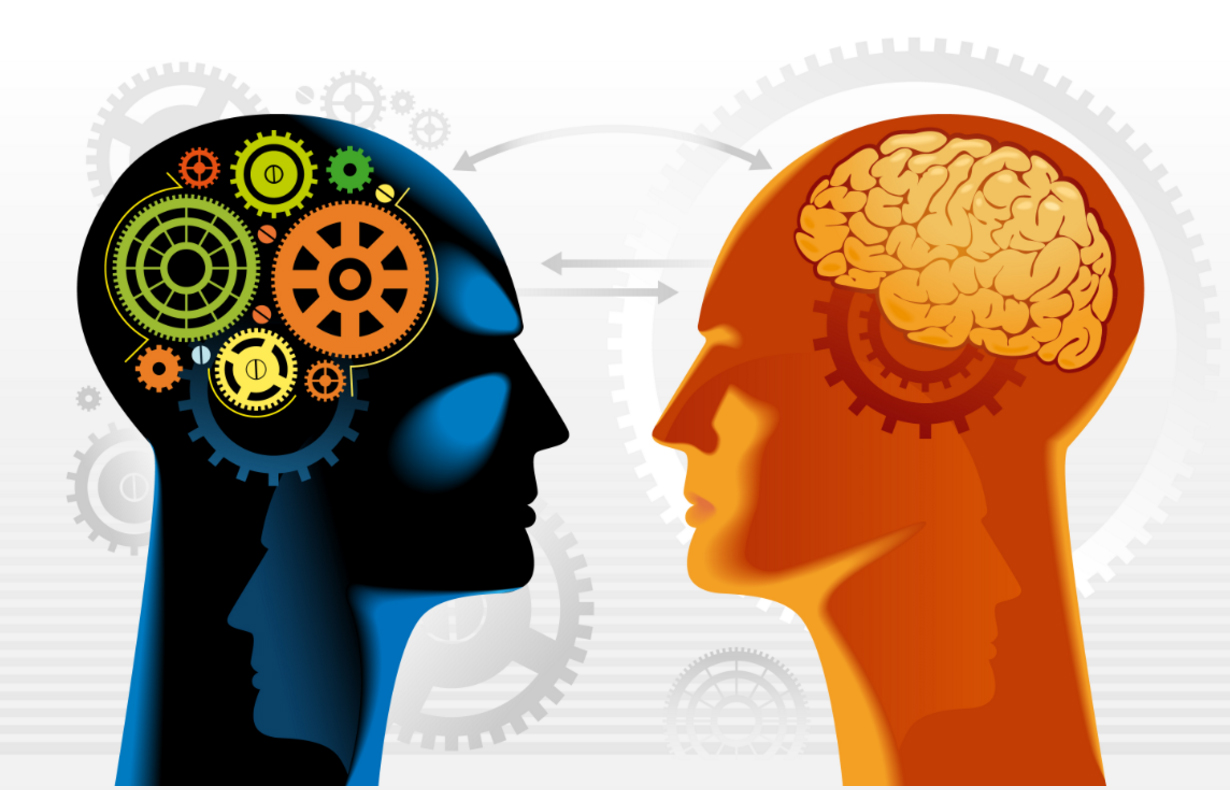
\includegraphics[width=0.25\textwidth]{ai_idea.jpg}
		\end{center}

		В 1832 г. российский изобретатель Семён Корсаков предложил серию <<интеллектуальных машин>>, работающих на перфокартах. В 1942 г. американский писатель Айзек Азимов в рассказе <<Хоровод>> сформулировал знаменитые правила поведения для роботов "--- три закона робототехники.
		\begin{center}
			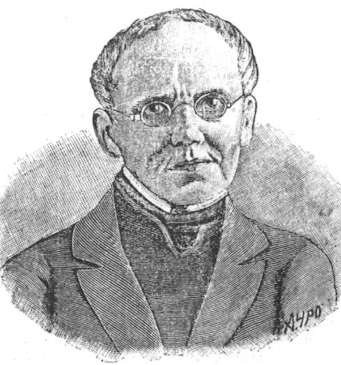
\includegraphics[height=0.25\textheight]{korsakov.jpg}\quad
			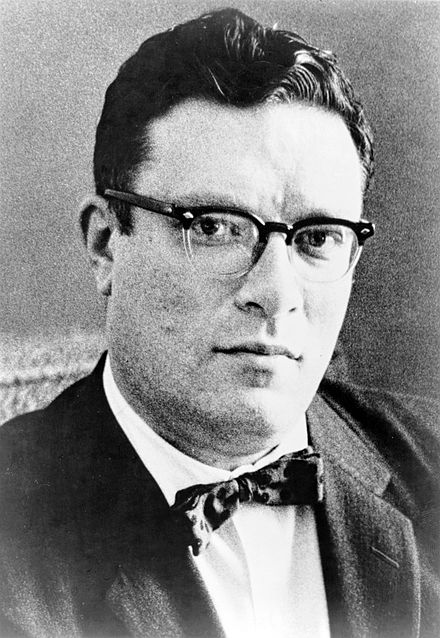
\includegraphics[height=0.25\textheight]{azimov.jpg}\quad
			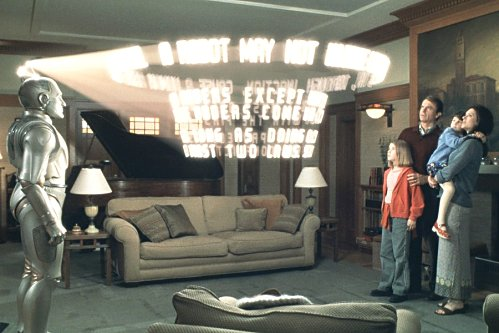
\includegraphics[height=0.25\textheight]{three_laws.jpg}
		\end{center}

		\textbf{Но возможна ли реализация этой идеи в принципе?}

	\end{frame}

	\begin{frame}
		\frametitle{Искусственный интеллект как мечта}
		\small
		В 1950 г. в философском журнале <<Mind>> появилась статья английского ученого Алана Тьюринга под названием <<Вычислительные машины и разум>> (Computing Machinery and Intelligence), в которой предложил знаменитый тест.
		\begin{center}
			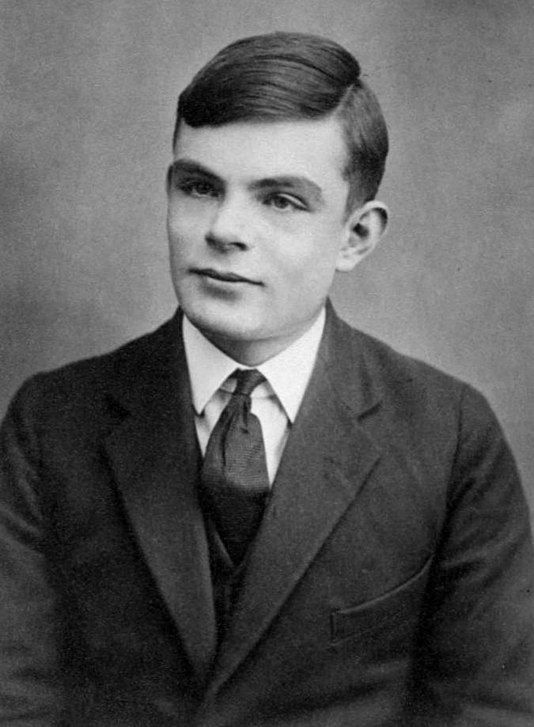
\includegraphics[height=0.27\textheight]{turing.jpg}\quad
			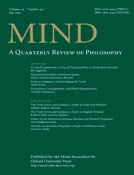
\includegraphics[height=0.27\textheight]{mind_journal.jpg}
		\end{center}		
		\footnotesize
		Аргументы против ИИ:
		\begin{itemize}
			\item \textbf{Теологический}: мышление как функция бессмертной души.
			\item \textbf{Этический}: последствия создания ИИ непредсказуемы. 
			\item \textbf{Математический}: теорема Гёделя и возражения Пенроуза.
			\item \textbf{Психологический}: что такое сознание.
			\item \textbf{Нейрофизиологический}: непрерывность нервной системы.
			\item \textbf{Экстрасенсорный}: отсутствие телепатии.
		\end{itemize}
		
		
	\end{frame}

	\begin{frame}
		\frametitle{Искусственный интеллект как мечта}
		\footnotesize
		Возможно ли создание машины, способной мыслить как человек?	Два ответа "--- две гипотезы:
		\begin{itemize}
			\item \textit{теория сильного искусственного интеллекта} предполагает, что компьютеры могут приобрести способность мыслить и осознавать себя, хотя и не обязательно их мыслительный процесс будет подобен человеческому.
			\item \textit{теория слабого искусственного интеллекта} отвергает такую возможность.
		\end{itemize}
		Мысленный эксперимент американского философа Джона Сёрла, предложенный им в 1980 г.
		\begin{center}
			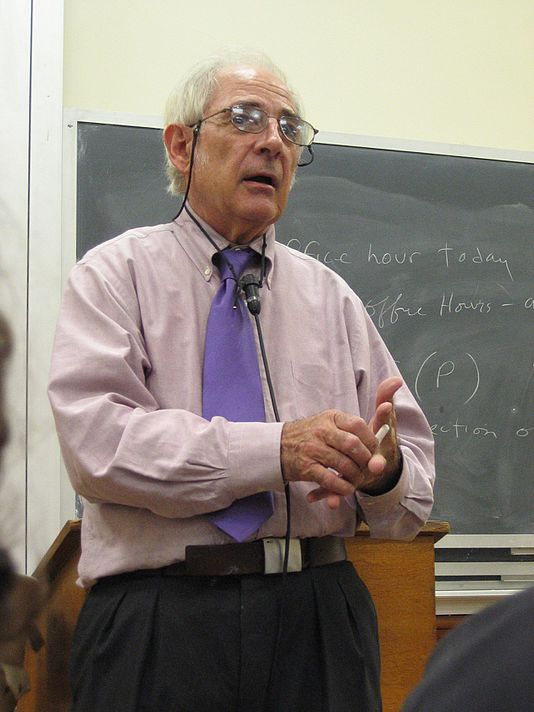
\includegraphics[height=0.4\textheight]{searle.jpg}\quad
			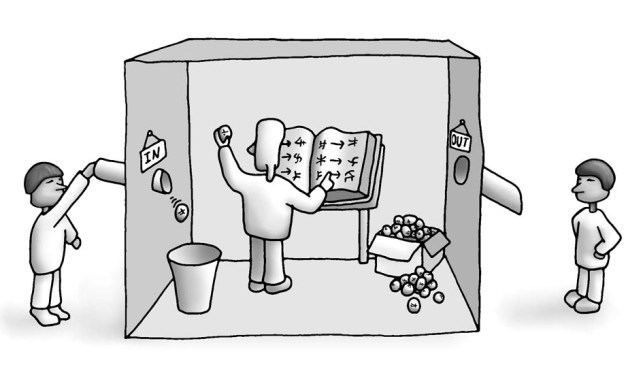
\includegraphics[height=0.4\textheight]{china_room.jpg}
		\end{center}
	\end{frame}

	\begin{frame}
		\frametitle{ИИ как научное направление}
		\small
		Определения искусственного интеллекта как научного направления:
		\onslide<1->{
		\begin{columns}
			\begin{column}{0.2\textwidth}
				\centering
				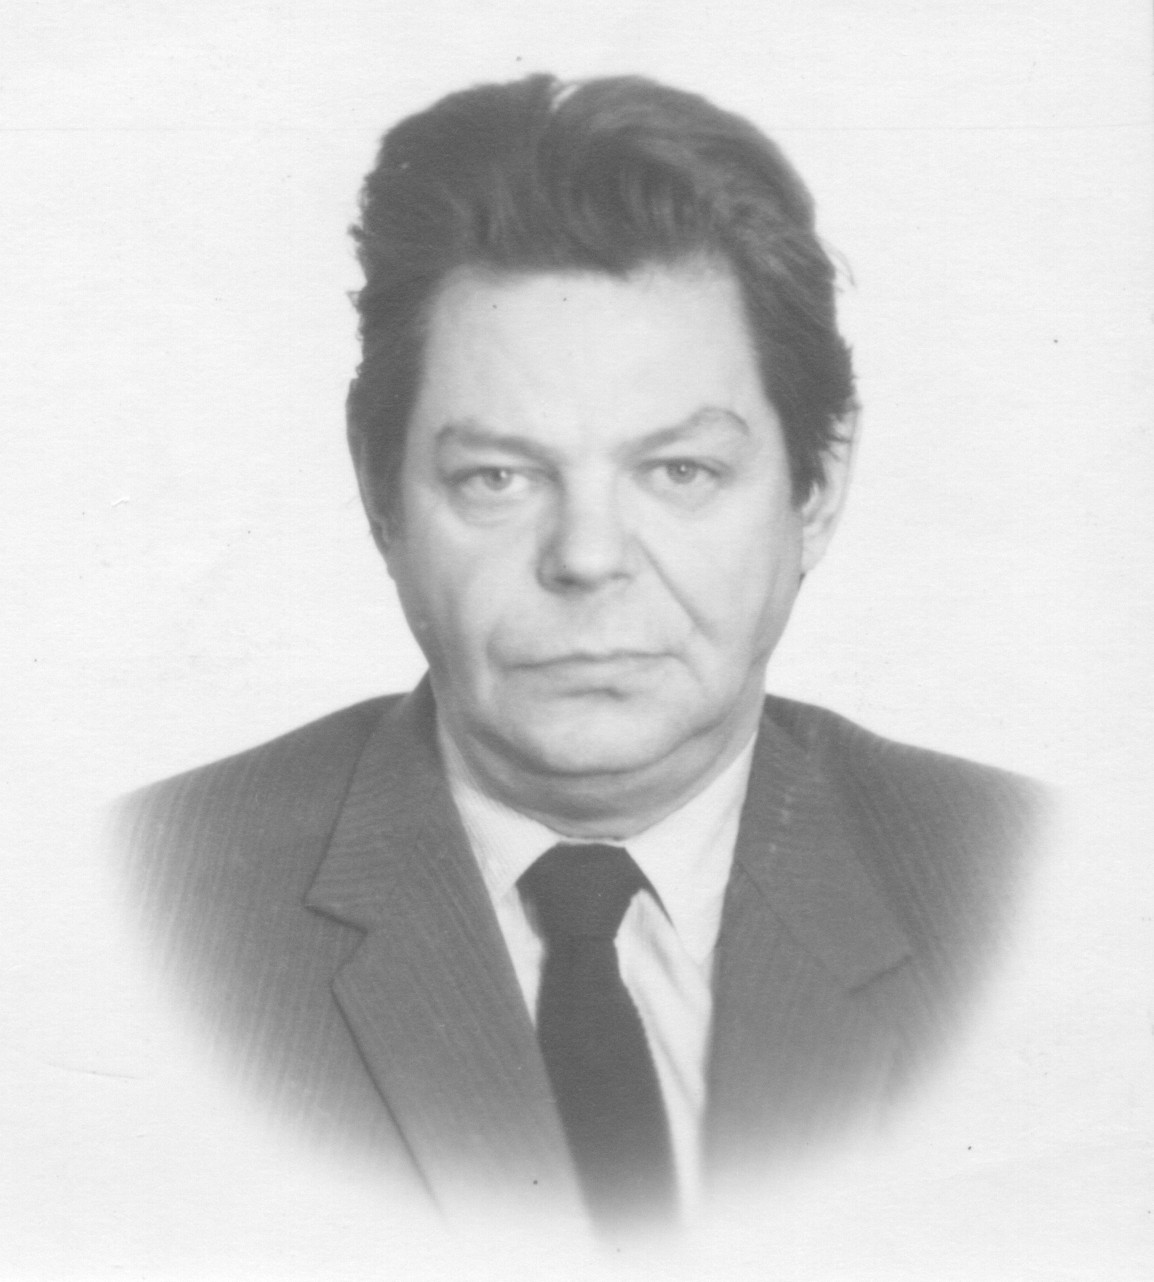
\includegraphics[width=\textwidth]{pospelov.png}
			\end{column}
			\begin{column}{0.8\textwidth}
				ИИ - это научное направление, в рамках которого ставятся и решаются задачи аппаратного или программного моделирования тех видов человеческой деятельности, которые традиционно считаются интеллектуальными (Дмитрий Поспелов).
			\end{column}
		\end{columns}
		}	
				
		\onslide<2->{
			\begin{columns}
				\begin{column}{0.2\textwidth}
					\centering
					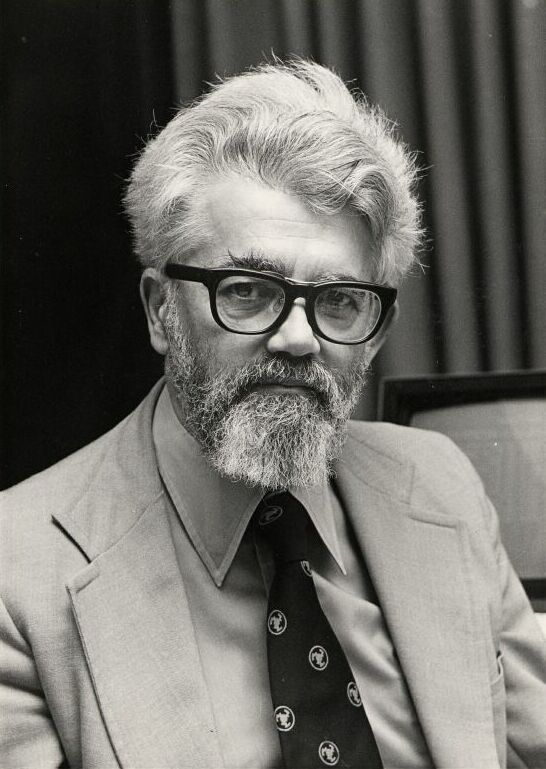
\includegraphics[width=0.8\textwidth]{mccarthy.jpg}
				\end{column}
				\begin{column}{0.8\textwidth}
					ИИ - это наука и технология создания интеллектуальных машин, особенно интеллектуальных компьютерных программ (Джон Маккарти).
				\end{column}
			\end{columns}
		}
		\onslide<3->{
			\begin{columns}
				\begin{column}{0.2\textwidth}
					\centering
					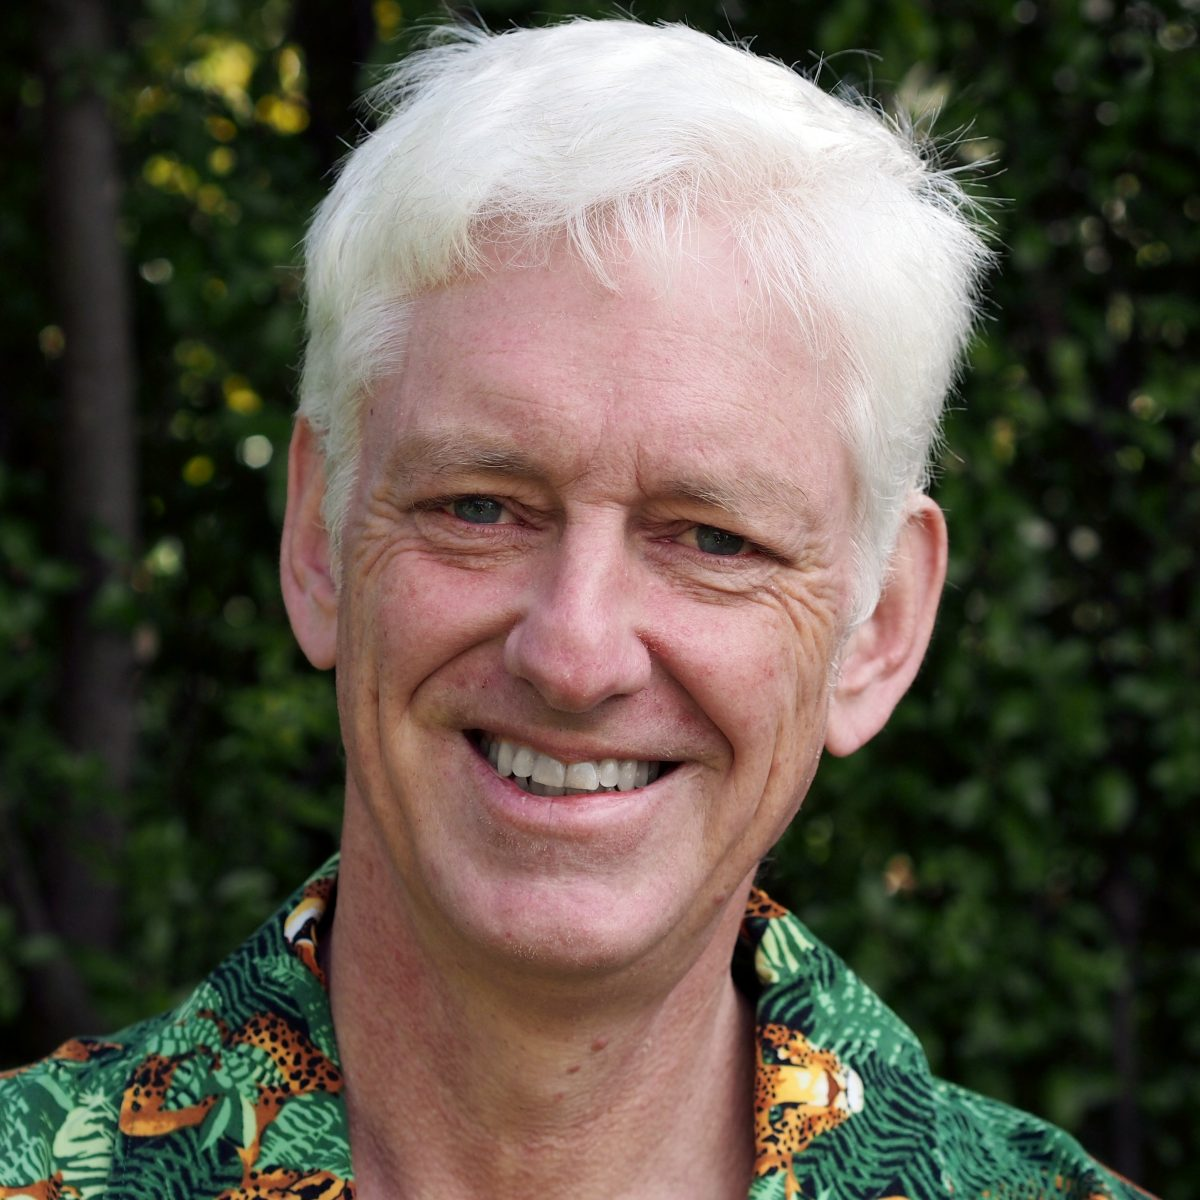
\includegraphics[width=\textwidth]{norvig.jpg}
				\end{column}
				\begin{column}{0.8\textwidth}
					ИИ - это наука об <<интеллектуальных агентах>>, т.е. о некотором устройстве или программе, которая воспринимает свою среду и выполняет действия, которые максимизируют ее шансы на успех при достижении какой-то цели (Питер Рассел).
				\end{column}
			\end{columns}
		}
	\end{frame}
	

	\begin{frame}
		\frametitle{Когнитивные науки}
		
		
		\centering
		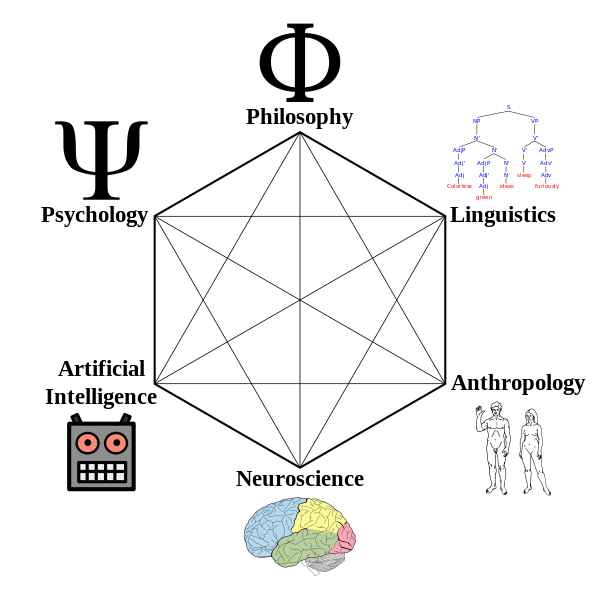
\includegraphics[width=0.5\textwidth]{cogsci.png}
		
		Когнитивная наука (лат. cognitio <<познание>>) - междисциплинарное научное направление изучающее психику, разум (mind) человека и реализующие его процессы.
	\end{frame}

	\section{Немного истории}
	\subsection{1.1}
	\begin{frame}
		\frametitle{Программная реализация ИИ}

		\begin{itemize}
			\item \textbf{1954 г.} --- аналитики \textit{Рэнд Корпорейшн}, \textit{Аллан Ньюэлл}, \textit{Дж. Шоу} и \textit{Герберт Саймон}  решили написать программу игры в шахматы. В этой затее им вызвались помочь \textit{А. Тьюринг} и \textit{К. Шеннон}, а также группа голландских психологов.
			\item \textbf{1956 г.} ---Дартмутский семинар (конференция по вопросам искусственного интеллекта, проведённая летом 1956 года в Дартмутском колледже).
			\item \textbf{1957 г.} --- программа для игры в шахматы (NSS) была написана. В основе работы NSS лежали эвристики --- правила выбора в отсутствие теоретических оснований.
		\end{itemize}
	\end{frame}
	\subsection{1.2}
	\begin{frame}
	\frametitle{Дальнейшее развитие}
	
		\begin{itemize}
			\item \textbf{1960 г.}  --- GPS (<<универсальный решатель задач>>, \textit{Аллан Ньюэлл}л и \textit{Герберт Саймон}): вычисление неопределенных интегралов, головоломки и  некоторые другие задачи.  Программы автоматического доказательства теорем из планиметрии, решения алгебраических задач. 
			\item \textbf{1960 г.} --- возникновение \textbf{эвристического программирования}. 
			\item \textbf{1963 г.} --- \textit{Джон Маккарти} --- ЛИСП. \textbf{Возникновение функционального программирования}.
			\item \textbf{1968 г.} --- книга <<Семантическая обработка информации>> \textit{Марвина Минского}.
		\end{itemize}
	\end{frame}
	\subsection{1.3}
	\begin{frame}
		\frametitle{Поиск непереборных методов решения задач}
		
		\begin{itemize}
			\item \textbf{1964 г.} --- \textit{В.Н. Пушкин} и \textit{Д.А. Поспелов}  --- модельная гипотеза мышления versus лабиринтной; методы решения переборных задач человеком. 
			\item \textbf{1964 г.} --- \textit{С.Ю. Маслов} --- метод автоматического поиска доказательства теорем в исчислении предикатов (обратный метод).
			\item \textbf{1965 г.} --- \textit{Дж.А. Робинсон} --- метод автоматического поиска доказательства теорем в исчислении предикатов (метод резолюций).
			\item \textbf{1968 г.} --- возникновение \textbf{логического программирования}.
			\item \textbf{1971 г.} --- \textit{А. Колменрауэр} --- \textbf{язык Пролог}.
			\item \textbf{1976 г.} --- Гипотеза \textit{Саймона} и \textit{Ньюэлла}: <<Физическая символьная система имеет необходимые и достаточные средства для произведения базовых интеллектуальных действий>>.
		\end{itemize}
	\end{frame}

	\subsection{1.4}

	\begin{frame}
		\frametitle{Современный ИИ}
		\centering
		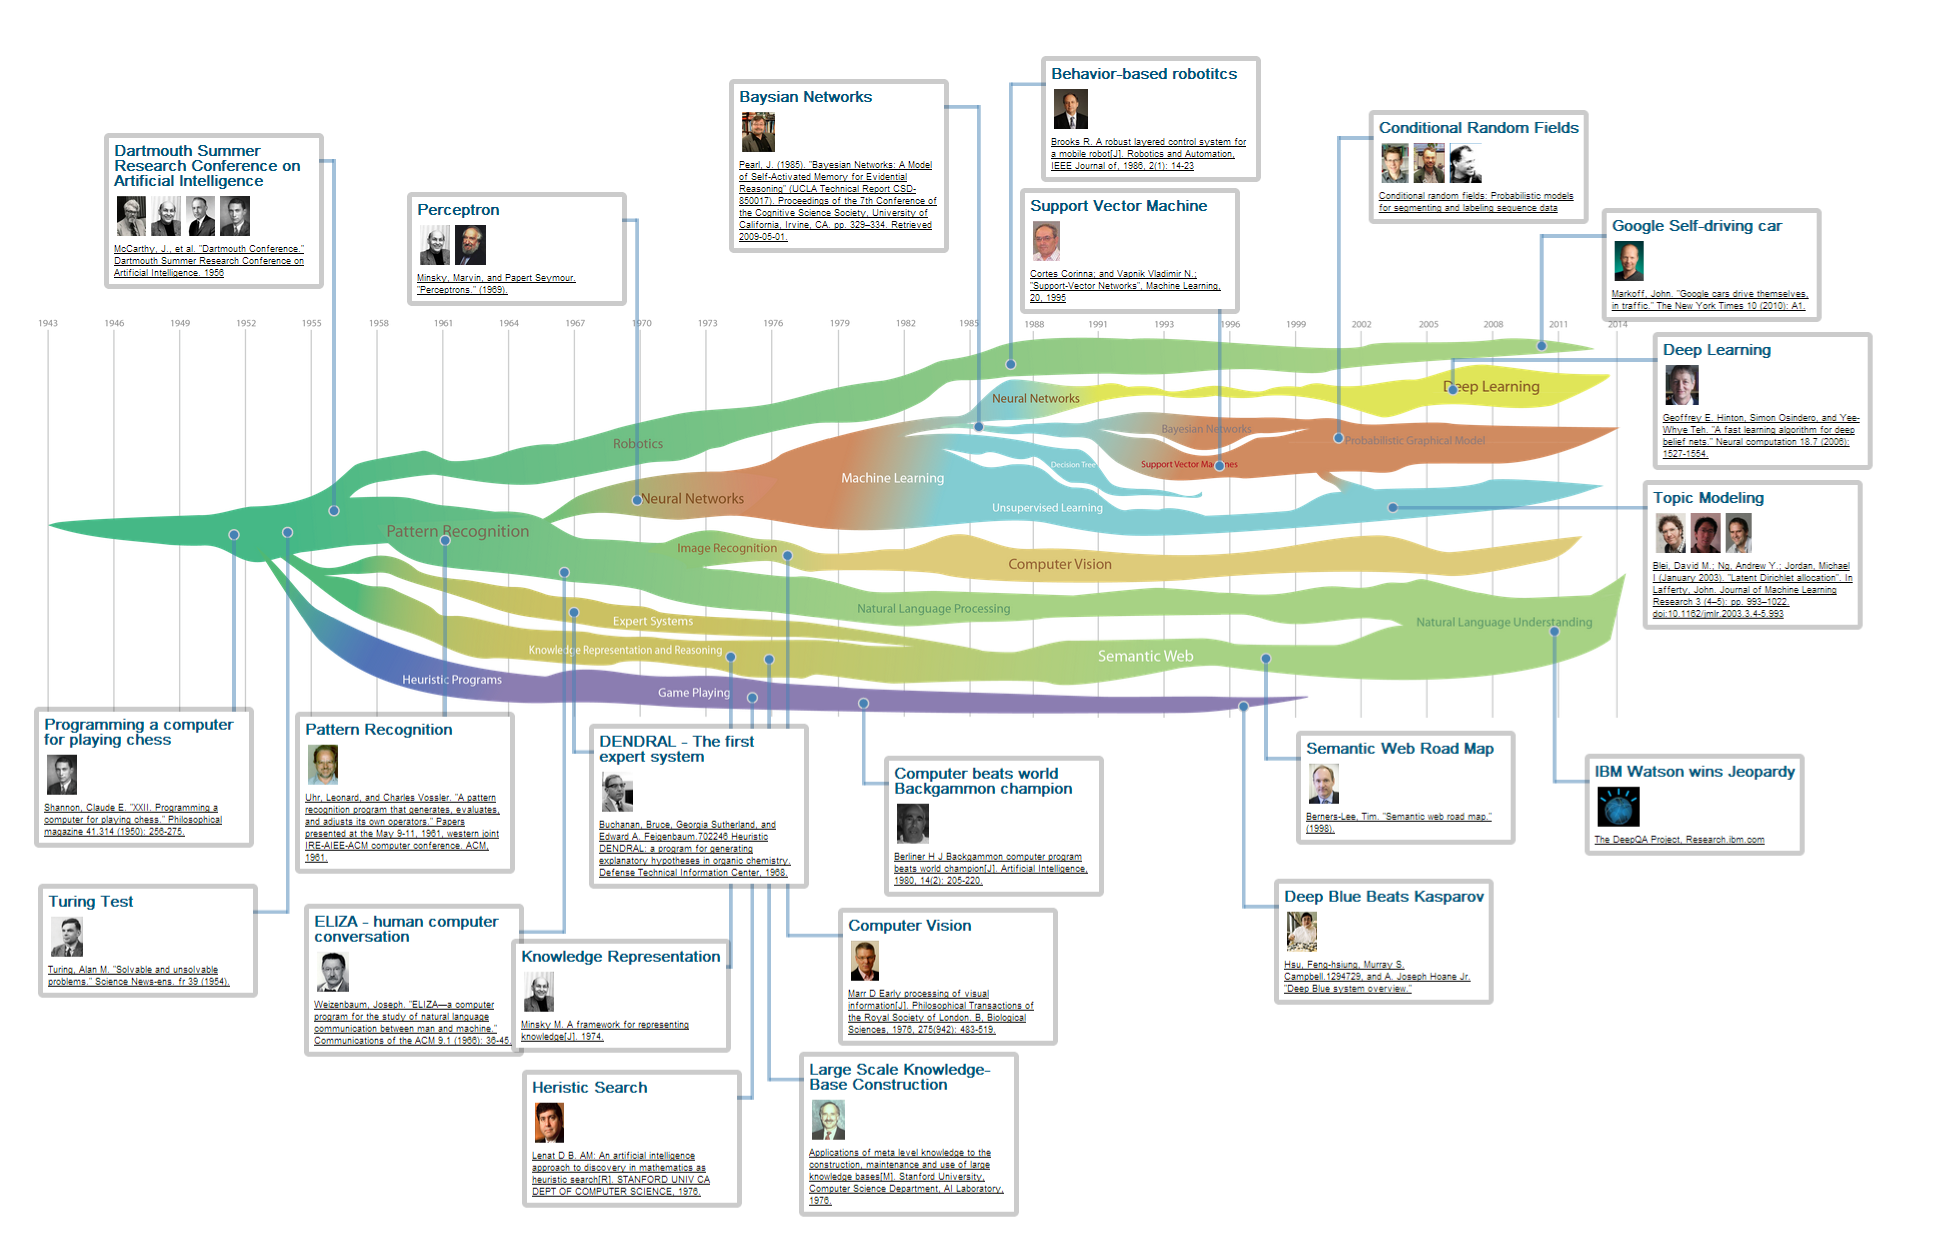
\includegraphics[width=1.15\textwidth]{ai-1.png}
	\end{frame}
	
	\begin{frame}
		\frametitle{Современный ИИ}
		Сформировались два основных подхода к разработке систем искусственного интеллекта:
		\begin{itemize}
			\item \textit{нисходящий} (Top-Down AI), символьный: создание экспертных систем, баз знаний и систем логического вывода, имитирующих высокоуровневые психические процессы: мышление, рассуждение, речь, эмоции, творчество и т. д.;
			\item \textit{восходящий} (Bottom-Up AI), биологический: изучение нейронных сетей и эволюционных вычислений, моделирующих интеллектуальное поведение на основе биологических элементов, а также создание соответствующих вычислительных систем.
		\end{itemize}
	
		\textbf{Перспективное направление - объединение}: знаковые системы, нейросимвольные вычисления.
	\end{frame}


	\section{Организация ИИ}
	\subsection{2.1}
	\begin{frame}
		\frametitle{Искусственный интеллект --- организационная структура}
		
		\begin{itemize}
			\item Во многих странах есть ассоциации искусственного интеллекта (EurAI,AAAI, RAAI).
			\item Каждый или раз в два года проходят крупнейшие конференции по ИИ: ECAI, AAAI Conference, IJCAI, КИИ.
			\item РААИ - общероссийская общественная организация (261 индивидуальный член, 45 региональных отделений).
			\item Выходят тематические журналы (Artificial Intelligence, Cognitive Psychology, Autonomous Robots, Neural Networks, Искусственный интеллект и принятие решений).
		\end{itemize}
		\par\bigskip
		\centering
		
\includegraphics[height=30pt]{aaai.png} \hspace{10pt}
		
\includegraphics[height=30pt]{eurai.png} \hspace{10pt}
		\includegraphics[height=30pt]{misc/logos/raai.png} 
	\end{frame}

	\subsection{2.2}
	\begin{frame}
		\frametitle{Источники}
		\scriptsize
		Онлайн: Coursera, Udacity, postnauka.ru, курсы ведущих университетов:
				\begin{itemize}
					\item Machine Learning and Artificial Intelligence в Принстоне (\url{https://www.cs.princeton.edu/courses/archive/fall16/cos402/})
					\item Artificial Intelligence в CMU (\url{http://www.cs.cmu.edu/~./15381/})
					\item Deep Learning for Self-Driving Cars в MIT (\url{http://selfdrivingcars.mit.edu})
					\item Deep Reinforcement Learning в Беркли (\url{http://rll.berkeley.edu/deeprlcourse/})
				\end{itemize}
		Книги:
			\begin{itemize}
				\item  Nilsson N.J. Artificial Intelligence: A New Synthesis. San Francisco: Morgan Kaufmann, 1998. 513 p.
				\item Russell S., Norvig P. Artificial Intelligence: A Modern Approach, Prentice Hall, 2009 (3 edition), P. 1152. (Искусственный интеллект. Современный подход)
				\item Осипов Г.С. Методы искусственного интеллекта. М.: ФИЗМАТЛИТ, 2011.
				\item Flreani D., Mattiussi C. Bio-Inspired Artificial Intelligence: Theories, Methods, and Technologies, The MIT Press, 2008, P. 658.
				\item Поспелов Д.А. Моделирование рассуждений. Опыт анализа мыслительных актов. М.: Радио и связь, 1989. 184 с.
				\item Гаазе-Рапопорт М.Г., Поспелов Д.А. От амебы до робота. Модели поведения. М.: Наука, 1987. 288 с.
				\item Что-то <<популярное>> (Джефф Хокинс, Сандра Блейксли. Об интеллекте; Роджер Пенроуз. Новый ум короля)
			\end{itemize}
	   Профессиональные интернет-ресурсы (\url{http://open.ai}, \url{https://deepmind.com})
	\end{frame}


	\section{Направления ИИ}
	\subsection{3.1}
	\begin{frame}
		\frametitle{Основные направления ИИ}
		\centering
		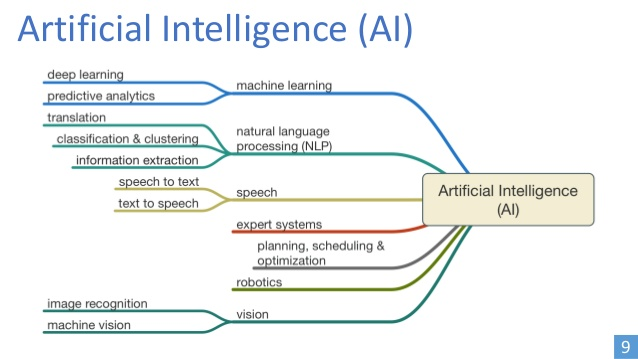
\includegraphics[width=\textwidth]{ai_fields.jpg}
	\end{frame}

	\begin{frame}
		\frametitle{Основные направления ИИ}
		\centering
		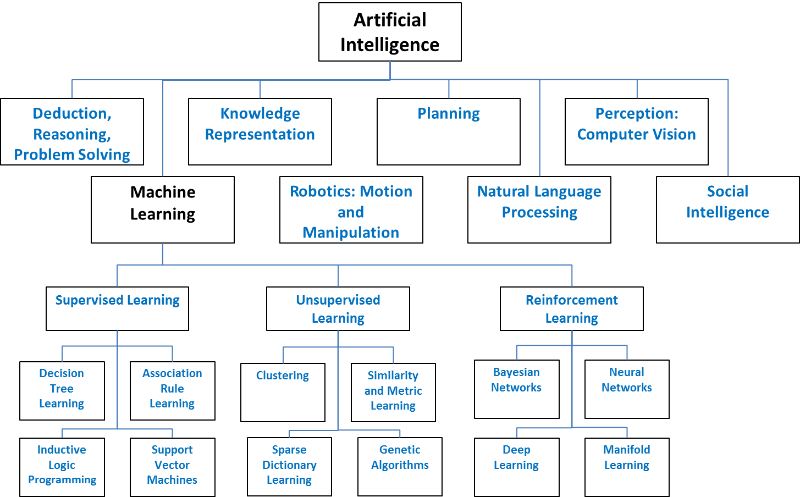
\includegraphics[width=\textwidth]{ai_fields3.png}
	\end{frame}

	\begin{frame}
		\frametitle{Основные направления ИИ}
		\centering
		\footnotesize
		\makebox[0.8\textwidth][c]{
			\begin{tikzpicture}
				\node[ellipse, minimum width = 100, minimum height = 50, fill=blue!20, align=center] (d1) {Искусственный\\интеллект};
				
				\node[rounded corners=5pt,draw,color=blue!20, very thick,text=black] (d2) at (-4,2) {
					\begin{minipage}[c][33pt]{100pt}
						\centering
						\textbf{Приобретение знаний, анализ данных и порождение гипотез}
					\end{minipage}
				};
				\node[rounded corners=5pt,draw,color=blue!20, very thick,text=black] (d3) at (-4,0.5) {
					\begin{minipage}[c][20pt]{80pt}
					\centering
					\textbf{Моделирование рассуждений}
					\end{minipage}
				};
	
				\node[rounded corners=5pt,draw,color=blue!20, very thick,text=black] (d4) at (-4,-0.7) {
					\begin{minipage}[c][20pt]{80pt}
					\centering
					\textbf{Многоагентные системы}
					\end{minipage}
				};
			
				\node[rounded corners=5pt,draw,color=blue!20, very thick,text=black] (d5) at (-4,-2.3) {
					\begin{minipage}[c][43pt]{110pt}
					\centering
					\textbf{Обработка естественного языка, пользовательский интерфейс и модели пользователя}
					\end{minipage}
				};
			
			
				\node[rounded corners=5pt,draw,color=blue!20, very thick,text=black] (d6) at (4,2) {
					\begin{minipage}[c][33pt]{120pt}
					\centering
					\textbf{Динамические интеллектуальные системы и планирование поведения}
					\end{minipage}
				};
				\node[rounded corners=5pt,draw,color=blue!20, very thick,text=black] (d7) at (4,0.5) {
					\begin{minipage}[c][20pt]{80pt}
					\centering
					\textbf{Представление знаний}
					\end{minipage}
				};
				
				\node[rounded corners=5pt,draw,color=blue!20, very thick,text=black] (d8) at (4,-0.7) {
					\begin{minipage}[c][20pt]{100pt}
					\centering
					\textbf{Нечеткие модели и мягкие вычисления}
					\end{minipage}
				};
				
				\node[rounded corners=5pt,draw,color=blue!20, very thick,text=black] (d9) at (4,-2.3) {
					\begin{minipage}[t][20pt]{110pt}
					\centering
					\textbf{Инструментальные средства и технологии}
					\end{minipage}
				};
				
				\draw[->,rounded corners=10pt, very thick, blue!20](d1)[xshift=-10] |- (d2.east);
				\draw[->,rounded corners=10pt, very thick, blue!20](d1)[xshift=10] |- (d6.west);
				
				\draw[->,rounded corners=10pt, very thick, blue!20](d1)[xshift=-10] |- (d5.east);
				\draw[->,rounded corners=10pt, very thick, blue!20](d1)[xshift=10] |- (d9.west);
				
				\draw[->,rounded corners=10pt, very thick, blue!20](d1) |- (d3.east);
				\draw[->,rounded corners=10pt, very thick, blue!20](d1) |- (d7.west);
				
				\draw[->,rounded corners=10pt, very thick, blue!20](d1.south west) |- (d8.west);
				\draw[->,rounded corners=10pt, very thick, blue!20](d1.south east) |- (d4.east);
			\end{tikzpicture}
		}
	\end{frame}

	\subsection{3.2}
	\begin{frame}
		\frametitle{Приобретение знаний, анализ данных и автоматическое порождение гипотез}
		
		\textbf{Цель}: создание методологий, технологий и программных средств обнаружения и переноса компетентности   в базы знаний.
		\par\medskip
		\centering
		\tikz[baseline]{
			\small
			\node[fill=yellow, rounded corners=5pt, minimum width=300, minimum height = 150] (k1) {
				\begin{minipage}[t][150pt]{300pt}
					\centering
					\textbf{Методы приобретения знаний:}
				\end{minipage}
				
			};
			
			\node[rounded corners=5pt, minimum width=280, minimum height = 50, text width= 250, text centered,fill=white] (k2) at (0, 0.85) {
				\begin{minipage}[t][60pt]{250pt}
					\centering
					\textbf{Машинное обучение и обучение по примерам} (методы построения деревьев решений,  индуктивные методы построения правил;  статистические методы, в частности, Байесовские  сети; метод ближайших соседей, искусственные нейронные сети)
				\end{minipage}
				
			};
		
			\node[rounded corners=5pt, minimum width=280, minimum height = 10, text width= 250, text centered,fill=white] (k2) at (0,-0.9) {
				\begin{minipage}[t][10pt]{250pt}
					\centering
					\textbf{Приобретение знаний из текстов}
				\end{minipage}
				
			};
		
			\node[rounded corners=5pt, minimum width=280, minimum height = 20, text width= 250, text centered,fill=white] (k2) at (0, -2) {
				\begin{minipage}[t][20pt]{250pt}
					\centering
					\textbf{Прямые методы приобретения знаний (автоматизированный диалог с экспертами)}
				\end{minipage}
				
			};
		}
	\end{frame}

	\subsection{3.3}
	\begin{frame}
		\frametitle{Представление знаний}
		
		\textbf{Предмет}:  разработка языков и программных средств   для описания экспертных и эмпирических знаний. 
		\par\medskip
		\textbf{Содержание}:
		\begin{itemize}
			\item семантические сети, системы фреймов, системы правил (продукционные системы) и их гибриды;
			\item логики пространства и времени;
			\item онтологии – способ обмена знаниями;
			\item дескриптивные логики (теория баз знаний и онтологий).
		\end{itemize}
	\end{frame}

	\subsection{3.4}
	\begin{frame}
		\frametitle{Автоматизация  рассуждений}
		
		Методы индукции, абдукции и аналогии, аргументации, рассуждения на основе прецедентов, на основе ограничений, рассуждения о действиях и изменениях, рассуждения с неопределенностью, немонотонные рассуждения.
		\par\medskip
		\tikz[baseline]{
			\node[fill=blue!20, rounded corners=5pt, anchor=base] (t1) {\textbf{Немонотонные рассуждения}};
		}
		связаны с поиском эмпирических зависимостей в данных, обучением по примерам и рассуждениями в эмпирических  теориях. Выделились в самостоятельный раздел логики.
		\par\medskip
		\tikz[baseline]{
			\node[fill=blue!20, rounded corners=5pt, anchor=base] (t2) {\textbf{Рассуждения о действиях}};
		}
		исследуют связь  действий и эффектов действий (результатов действий).
		\par\medskip
		\tikz[baseline]{
			\node[fill=blue!20, rounded corners=5pt, anchor=base] (t3) {\textbf{Рассуждения с неопределенностью}};
		}
		--- использование  Байесовского  формализма в моделях рассуждений. 
		
	\end{frame}

	\subsection{3.5}
	\begin{frame}
		\frametitle{Многоагентные системы}
		
		Изучаются интеллектуальные программные агенты, их коалиции и поведение.
		
		\par\medskip
		\textbf{Интеллектуальный программный  агент} --- программная система, обладающая автономностью, социальными чертами, реактивностью и активностью.
		
		\par\medskip
		\textbf{Основные проблемы}: коммуникация интеллектуальных агентов, разработка языков для этой цели, координация поведения  агентов, распределение ролей в коалициях агентов, коллективное поведение агентов.
	\end{frame}

	\subsection{3.7}
	\begin{frame}
		\frametitle{Роботы и автономные системы}
		\Large
		\begin{itemize}
			\item Диалоговое взаимодействие коалиций мобильных роботов.
			\item Интерпретация команд, поступающих от человека.
			
			\item Качественные логики пространства-времени.
			
			\item Рассуждения, основанные на оценках.
			
			\item Проблема символизации (symbol grounding problem).
		\end{itemize}
		
	\end{frame}

	\subsection{3.8}
	\begin{frame}
		\frametitle{Интеллектуальные динамические системы и автоматическое планирование поведения}
		\Large
		
		\textbf{Результат интеграции} методов искусственного интеллекта с теорией динамических систем:
		\begin{itemize}
			\item планирование,
			\item моделирование,
			\item управление.
		\end{itemize}
		
	\end{frame}

	%\subsection{3.9}
	\begin{frame}
		\frametitle{Обработка естественного языка, интерфейс и модели пользователя}
		\begin{itemize}
			\small
			\item Семантический поиск в больших массивах текстов:
			\begin{itemize}
				\footnotesize
				\item поиск документов (в полнотекстовой БД, в локальных и глобальных телекоммуникационных сетях);
				\item извлечение данных из текстов;
				извлечение знаний из текстов.
			\end{itemize}
			
			\item Обработка текстов: сегментация, классификация, кластеризация, аннотирование или реферирование текстов. Перевод. 
			\item Диалоговые системы: 
			\begin{itemize}
				\footnotesize
				\item интеллектуальные вопросно-ответные системы; 
				\item системы общения конечных пользователей с БД, предоставляющие  различные услуги (выполнение банковских операций по телефону, заказ товаров по каталогам); 
				\item голосовое управление техникой, кооперативное решение проблем (человек плюс интеллектуальная система).
			\end{itemize}
			
			\item Автоматическое обучение анализу текстов.
			
		\end{itemize}
		
	\end{frame}

	\subsection{3.10}
	\begin{frame}
		\frametitle{Нечеткие модели и мягкие вычисления}
		
		\Large 
		\begin{itemize}
			\item Нечеткие схемы вывода по аналогии;
			\item теория нечетких мер; 
			\item модели геометрических объектов;
			\item алгоритмы эволюционного моделирования с динамическими параметрами (например, время жизни и размер популяции);
			\item методы решения оптимизационных задач с использованием технологий генетического поиска, гомеостатических и синергетических принципов и элементов самоорганизации. 
		\end{itemize}
		
	\end{frame}

	\subsection{3.11}
	\begin{frame}
		\frametitle{Вклад ИИ в другие  науки}
		
		Развитие ИИ привело к \textbf{возникновению самостоятельных областей}:
		\begin{itemize}
			\item эвристическое программирование,
			\item функциональное программирование,
			\item логическое программирование,
			\item объектно-ориентированное программирование,
			\item теория немонотонных рассуждений и немонотонные логики,
			\item инженерия знаний,
			\item технология программирования, основанная на знаниях,
			\item прикладная семиотика.
		\end{itemize}
		
		В \textbf{инженерном направлении}:
		\begin{itemize}
			\item экспертные системы.
		\end{itemize}
	\end{frame}

	\section{Перспективы ИИ}
	\subsection{4.1}
	\begin{frame}
		\frametitle{Перспективные направления ИИ}
		
		\begin{itemize}
			\item \textbf{Рассуждения, основанные на прецедентах}.
			\item \textbf{Рассуждения о пространстве} --- возрастающее значение для автономных мобильных устройств, анализа изображений (в частности, аэрофотоснимков), синтеза текстовых описаний по изображениям.
			\item \textbf{Методы машинного обучения и автоматического формирования гипотез} --- решение практических задач: от обнаружения  закономерностей в данных до повышения степени адаптивности различных технических устройств.
			\item Подходы, основанные на \textbf{технологии интеллектуальных агентов} перспективны при разработке больших программных систем.
			
		\end{itemize}
		
	\end{frame}

	\subsection{4.2}
	\begin{frame}
		\frametitle{Перспективные направления ИИ}
		
		\begin{itemize}
			\item \textbf{Влияние идей и методов ИИ на машинный анализ текстов на естественном языке} --- коснется  семантического анализа и методов синтаксического анализа --- в этой области оно проявится в учете модели мира и использовании знаний о предметной области  для уменьшения переборов  на более ранних стадиях анализа.
			\item \textbf{Понимание текста}.
			\item \textbf{Автоматическое планирование и управление поведением}. Область применения  - от бытовой  техники до беспилотных аппаратов для исследования глубокого космоса.
		\end{itemize}
		
	\end{frame}

	\subsection{4.4}
	\begin{frame}
		\frametitle{Проблемы}
		
		\begin{itemize}
			\item Переход от моделирования структурной организации к моделированию ментальных представлений, в частности, когнитивных функций, иначе говоря,от искусственного интеллекта --- к искусственному сознанию.
			\item Автоматическое (или полуавтоматическое) формирование интеллектуальными агентами модели мира, включая зрительные и слуховые образы предметов и их назначение.

		\end{itemize}
		
	\end{frame}

	\section{Прикладной ИИ}
	\subsection{5.1}
	\begin{frame}
		\frametitle{ИИ в индустрии}
		\centering
		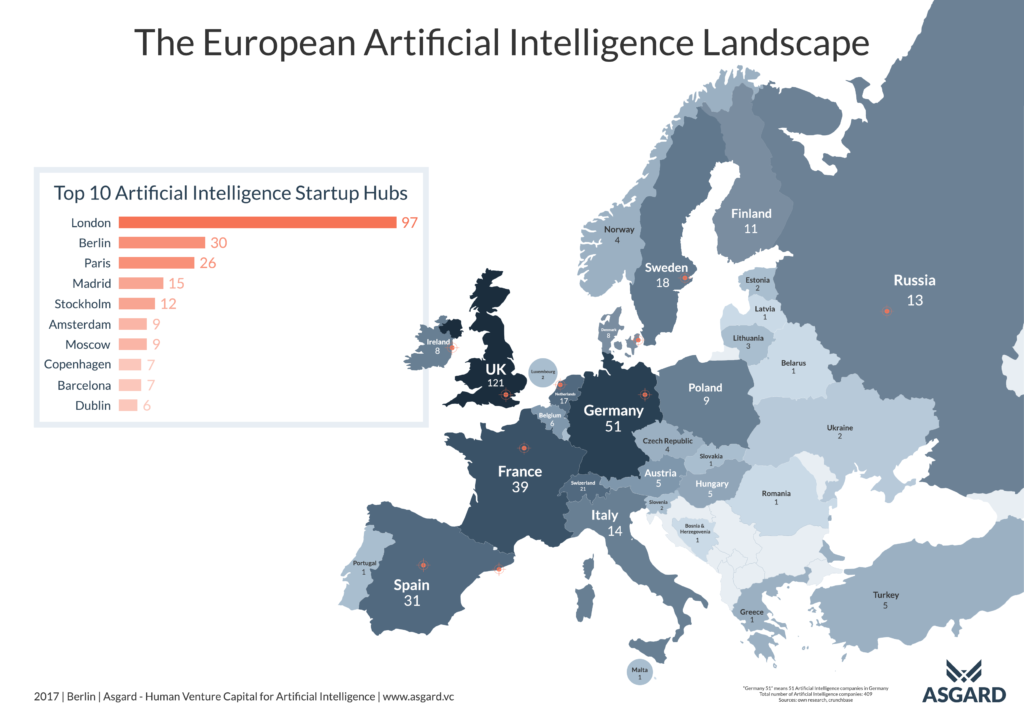
\includegraphics[width=0.6\textwidth]{asgard_1.png}
		\par\bigskip
		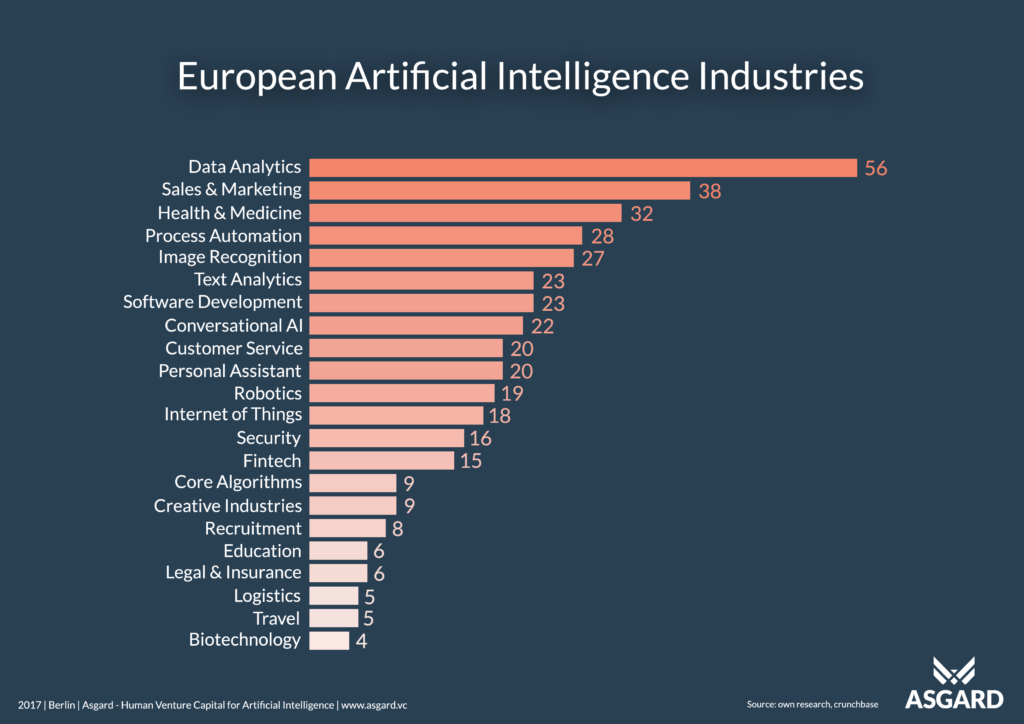
\includegraphics[width=0.3\textwidth]{asgard_2.png}
	\end{frame}

	\begin{frame}
		\frametitle{ИИ стартапы}
		\centering
		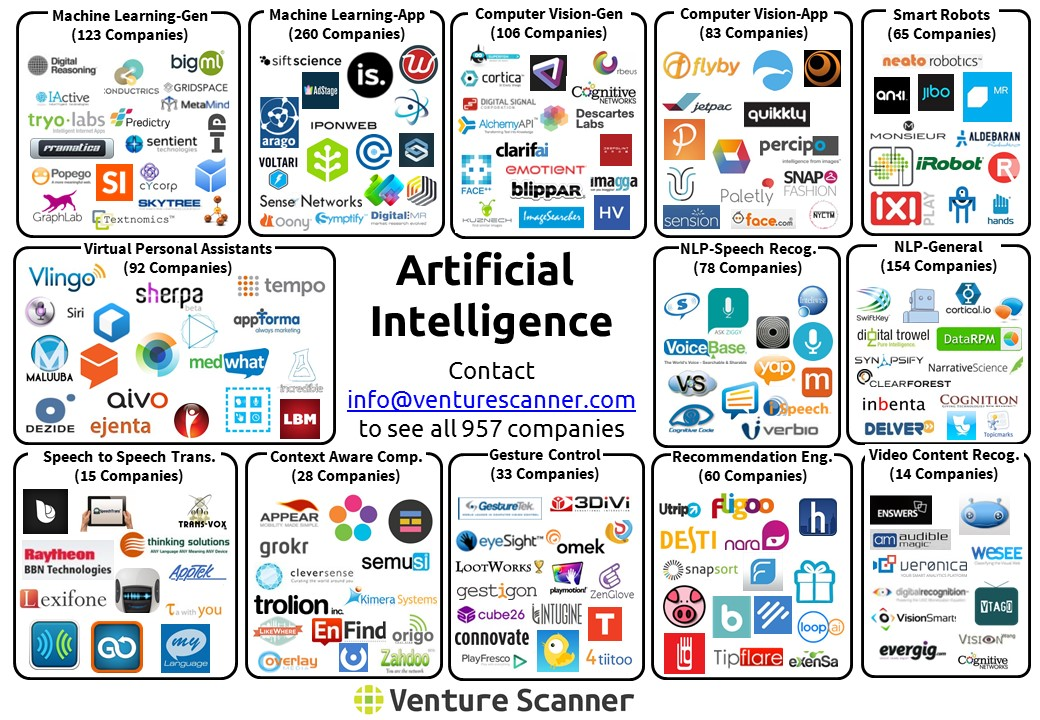
\includegraphics[width=\textwidth]{ai_startups.jpg}
	\end{frame}

	\begin{frame}
		\frametitle{Финансирование ИИ}
		\centering
		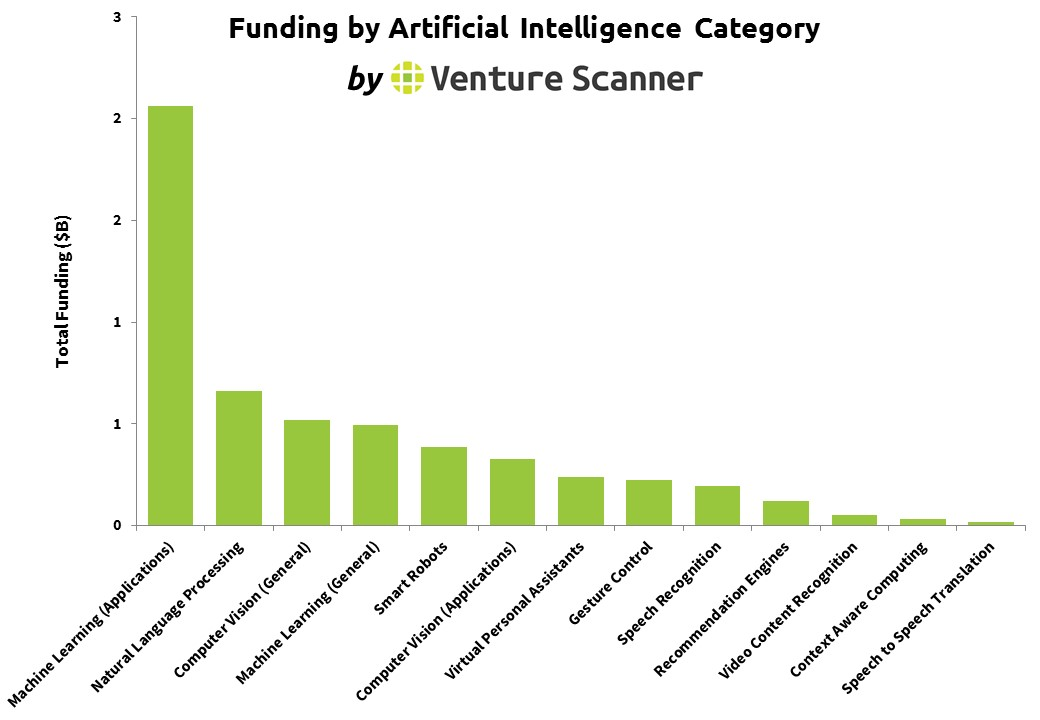
\includegraphics[width=0.9\textwidth]{ai_fund.jpg}
	\end{frame}

	\subsection{5.2}
	\begin{frame}
		\frametitle{Некоторые результаты в России}

		\begin{itemize}
			\item Разработан комплекс моделей поддержки принятия решений в конфликтных ситуациях с использованием когнитивных карт (ИПУ РАН). 
			\item Для модели летательного аппарата <<Этап>>	разработана теория бортовых 	интеллектуальных систем тактического уровня (БИС-Т/У), решающих задачи оперативного целеполагания и конструирования способа достижения оперативно назначенной цели (ГосНИИАС).
			\item Созданы роботы, архитектура системы управления которых включает эмоциональную компоненту (НИЦ <<Курчатовский институт>>). 
			\item Разработаны технологии поддержки интеллектуальных роботов-манипуляторов, способных автоматически принимать решения непосредственно во время работы (ИПМ РАН).
		\end{itemize}
	\end{frame}

	\begin{frame}
		\frametitle{Некоторые результаты в ФИЦ ИУ РАН}
		
		\begin{itemize}
			\item Создана семантическая поисковая машина нового поколения EXACTUS.  Машина работает с запросами на естественном языке.
			\item Неоднократно занимала первые места по релевантности поиска на соревнованиях поисковых 	машин \href{www.exactus.ru}{www.exactus.ru}.
			\item Создана система прогнозирования социального стресса на основе анализа социальных медиа.
			\item Созданы системы
			\begin{itemize}
				\item EXACTUS EXPERT --- для cемантического поиска и анализа качества научных публикаций,
				\item EXACTUS PATENT --- для семантического поиска и анализа патентной информации.
				\item EXACTUS LIKE для обнаружения близких текстов и вычисления степени семантической близости;
				\item TEXT Appliance --- информационно-аналитическая система анализа неструктурированной информации.
			\end{itemize}
		\end{itemize}
	\end{frame}

	\begin{frame}
		\frametitle{Архитектура STRL}
		\centering
		\includegraphics[width=0.7\textwidth]{agent-schemas/ru/architecture}
	\end{frame}
	
	\begin{frame}
		\frametitle{Картина мира субъекта деятельности}
		\scriptsize
		Картина мира субъекта деятельности - это представления субъекта о внешней среде, о своих собственных характеристиках, целях, мотивах, о других субъектах и операции (произвольные и непроизвольные), осуществляемые на основе этих представлений.
		\par\smallskip
		Элементом картины мира является знак:
		\begin{itemize}
			\item в смысле культурно-исторического подхода Выготского-Лурии,
			\item выполняющий функции в соответствии с теорией деятельности Леонтьева.
		\end{itemize}
		\begin{columns}
			\begin{column}{0.4\textwidth}
				\centering
				\includegraphics[width=0.6\textwidth]{signs/ru/sign_color_book_ru}
			\end{column}
			\begin{column}{0.6\textwidth}
				\begin{columns}
					\begin{column}{0.5\textwidth}
						\centering
						\includegraphics[width=\textwidth]{misc/phisio/ivan_cyrc}
					\end{column}
					\begin{column}{0.5\textwidth}
						\centering
						\includegraphics[width=\textwidth]{misc/phisio/workspace}
					\end{column}
				\end{columns}
				
			\end{column}
		\end{columns}
		В пользу существования такой структуры свидетельствуют:
		\begin{itemize}
			\item нейрофизиологические данные (Эдельман, Иваницкий, Маунткастл и др.),
			\item другие психологические теории (например, трехкомпонентная модель Станович).
		\end{itemize}
		\vspace{-5pt}
		\nocite{*}
		\printbibliography[keyword={sign}, resetnumbers=true]
		\end{frame}
		
	\begin{frame}
		\frametitle{Три образующих элемента картины мира}
		\vspace{-15px}
		\scriptsize
		\begin{columns}
		\begin{column}{0.6\textwidth}
			\begin{center}
				\includegraphics[width=0.3\textwidth]{signs/ru/sign_colored}
			\end{center}
			\vspace{-5pt}
			Представляемая сущность описывается тремя причинно-следственными (каузальными) структурами:
			\begin{itemize}
				\item {\color{red}структура образа} - представление взаимосвязи внешних сигналов и внутренних характеристик субъекта (агента) - сенсо-моторное представление,
				\item {\color{blue}структура значения} - обобщенное знание о соотношениях во внешнем мире, согласованное в некоторой группе субъектов (агентов),
				\item {\color{green!60!black}структура личностного смысла} - ситуационная потребностно-мотивационная интерпретация знаний о соотношениях во внешней среде (значение для себя).
			\end{itemize}
		\end{column}
		\begin{column}{0.4\textwidth}
			\begin{center}
				\includegraphics[width=0.5\textwidth]{signs/en/sign_naming_colored_en}
			\end{center}
			\textbf{Процесс обучения} "--- образование новых знаков как неподвижной точки операторов замыкания 
			\[\Psi_p^m\Psi_m^a\Psi_a^p.\]
			\par\smallskip
			Реализация когнитивных функций "--- \textbf{актуализация} (активация) имеющихся знаков и формирование новых <<ситуационных>> знаков "--- <<протознаков>> без конвенционального имени.
		\end{column}
		\end{columns}
	\end{frame}	

	\section*{}
	{
	\setbeamertemplate{headline}{}
	\begin{frame}
		\centering
		\Huge
		Спасибо за внимание!
		\normalsize
		\par\bigskip
		\par\bigskip
		МФТИ
		
		\par\bigskip
		panov.ai@mipt.ru
	\end{frame}			
	}
\end{document}
	
	
